\documentclass[francais,RandD]{rapportPFE}
\usepackage{listings}
\usepackage{fancyhdr}
\usepackage{amssymb}
\usepackage{amsmath}
\usepackage{amsfonts}
\usepackage[ruled,linesnumbered]{algorithm2e}
\usepackage{indentfirst}
\usepackage{graphicx}
\usepackage{subcaption}
\usepackage{xcolor}

\definecolor{codegreen}{rgb}{0,0.6,0}
\definecolor{codegray}{rgb}{0.5,0.5,0.5}
\definecolor{codepurple}{rgb}{0.58,0,0.82}
\definecolor{backcolour}{rgb}{0.95,0.95,0.92}
\lstdefinestyle{mystyle}{
    backgroundcolor=\color{backcolour},
    commentstyle=\color{codegreen},
    keywordstyle=\color{magenta},
    numberstyle=\tiny\color{codegray},
    stringstyle=\color{codepurple},
    basicstyle=\footnotesize,
    breakatwhitespace=false,
    breaklines=true,
    captionpos=b,
    keepspaces=true,
    numbers=left,
    numbersep=5pt,
    showspaces=false,
    showstringspaces=false,
    showtabs=false,
    tabsize=2
}
\lstset{
	basicstyle=\ttfamily,
	columns=fullflexible,
	frame=single,
	breaklines=true,
	postbreak=\mbox{\textcolor{red}{$\hookrightarrow$}\space},
	style=mystyle
}

\SetKwComment{Comment}{/* }{ */}

\fancyhf{}
\renewcommand{\headrulewidth}{0.2pt}
\renewcommand{\footrulewidth}{0.2pt}
\fancyhead[L]{\footnotesize{Un exemple d'en-têtes et pieds de page}}
\fancyfoot[R]{\thepage}
\fancyfoot[C]{\footnotesize{---}}
\fancyfoot[L]{\footnotesize{\textit{Les rédacteurs de la FAQ}}}

\newcommand{\TODO}[1]{\textcolor{red}{\textbf{TODO: #1}}}
\newcommand{\INFO}[1]{\textcolor{blue}{\textbf{INFO: #1}}}

\titre{Navigation et contrôle multi-robots pour l'inspection acoustique de structures métalliques}
\title{Multi-robot navigation and control for acoustic inspection of metal plate structures}
\firstname{Brandon}
% \middlename{Jérémy}
\lastname{Alves}
\dateDebutPFE{9 janvier 2023}
\dateFinPFE{30 juin 2023}
\nomStructureAcceuil{INRIA}
\villeStructureAccuel{Villeurbanne, France}
\logoStructureAccueil{width=4.5cm}{graphics/LogoStructureAccueil}
\begin{encadrants}
	\referent{Référent}{Cédric \Nom{Pradalier}}{Professeur}{GT Europe}
	\referent{Référent}{Olivier \Nom{Simonin}}{Professeur}{INSA Lyon}
	\tuteur{Tuteur}{Mathieu \Nom{Maranzana}}{Maître de conférences}{INSA Lyon}
\end{encadrants}
\date{27 juin 2023}

\begin{document}
	\maketitle
	\begin{ResumeMotsCles}
		\begin{resumeEn}
			This project is part of the European project BugWright2, which aims to address the problem of inspecting large metal structures using heterogeneous fleets of mobile robots. The project will focus on developing navigation strategies for mobile robots using guided ultrasonic waves to perform the inspection of metal plates. Guided waves have the ability to propagate along a plate by interacting with the material that makes it up and being affected by changes in geometry, such as corrosion. By combining measurements between a transmitter and a distant receiver system, it is possible to perform a tomography of the area to be inspected and potentially identify and locate points of corrosion.
		\end{resumeEn}
		\keywords{Navigation~; Multi-Robot~; Tomography~; Ultrasonic Guided Waves~; Inspection.}
		\begin{resumeFr}
			Ce projet fait partie du projet européen BugWright2 qui a pour objectif de résoudre la problématique de l'inspection de grandes structures métalliques en utilisant des flottes hétérogènes de robots mobiles. Le projet se concentrera sur le développement de stratégies de navigation pour des robots mobiles utilisant des ondes ultrasoniques guidées pour réaliser l'inspection de plaques métalliques. Les ondes guidées ont la capacité de se propager le long d'une plaque en interagissant avec la matière qui la compose et en étant affectées par des changements de géométrie, tels que la corrosion. En combinant des mesures entre un système émetteur et un système récepteur distant, il est possible de réaliser une tomographie de la zone à inspecter et de potentiellement identifier et localiser des points de corrosion.
		\end{resumeFr}
		\motscles{Navigation~; Multi-Robot~; Tomographie~; Ondes Guidées Ultrasoniques~; Inspection.}
	\end{ResumeMotsCles}
	\begin{remerciements}
		\TODO{Remerciements}
	\end{remerciements}
	\setcounter{tocdepth}{3}
	\listoffigures
	\listoftables
	\listofalgorithms
	\clearpage
	\tableofcontents
	\cleardoublepage
	\INFO{Ceci est un rapport d'environ 30 pages (hors annexes, hors première, deuxième, troisième et quatrième de couverture, hors table des matières et éventuelles autres tables des figures, des définitions, des algorithmes\ldots).}
	\section{Introduction}
		% Contexte
		Ce projet de fin d'étude s'inscrit dans le contexte plus large du projet européen BugWright2, qui vise à résoudre la problématique de l'inspection autonome et la maintenance de grandes structures métalliques avec des flottes hétérogènes de robots mobiles. Dans ce projet, nous nous concentrons sur le développement de stratégies de navigation pour un ensemble de robots mobiles utilisant des ondes ultrasoniques guidées pour réaliser l'inspection des plaques métalliques. En effet, les ondes guidées ont la particularité de se propager le long d'une plaque en interagissant avec la matière qui la compose, et en étant affectées par des changements de géométrie liés, en particulier, à la corrosion.

		% Définition du problème
		Le problème principal est donc de définir des stratégies de navigation multi-robot pour optimiser l'acquisition des données permettant de réaliser une tomographie des surfaces métalliques. Pour atteindre cet objectif, nous allons dans un premier temps effectuer une recherche bibliographique, puis mettre en place des méthodes de navigation dans un environnement de simulation. Enfin, nous envisagerons un déploiement sur différents robots en fonction des résultats obtenus. Ce projet sera réalisé sous la supervision de Olivier Simonin (INSA Lyon CITI lab) et de Cédric Pradalier (CNRS IRL2958 GT).

		% Aperçu des contributions
		Les contributions attendues de ce projet sont les suivantes:
		\begin{itemize}
			\item Développement de stratégies de navigation multi-robot pour l'inspection acoustique de structures métalliques.
			\item Optimisation de l'acquisition de données pour la réalisation de la tomographie.
			\item Résolution des problèmes de coordination entre les robots et de synchronisation des horloges.
			\item Implémentation des méthodes de navigation dans un environnement de simulation et leur déploiement sur des robots réels.
		\end{itemize}

		% Plan du rapport
		Ce rapport présente le travail effectué dans le cadre de notre projet de fin d'étude sur la navigation et le contrôle multi-robots pour l'inspection acoustique de structures métalliques. Dans la première section, nous introduisons le sujet du rapport et présentons les objectifs de notre projet. La deuxième section est consacrée à l'étude bibliographique, où nous résumons les recherches et les publications existantes sur le sujet. Dans la troisième section, nous proposons une solution pour la navigation et le contrôle multi-robots pour l'inspection acoustique de structures métalliques. Cette section est divisée en trois sous-sections : définitions préliminaires, proposition de solution et étude théorique de propriétés de la solution proposée. La quatrième section décrit les détails de l'implémentation technique de notre solution proposée. La cinquième section présente les résultats de nos expérimentations, validations et évaluations. Dans la sixième section, nous faisons un bilan personnel de notre expérience de travail sur ce projet. Enfin, dans la septième section, nous concluons notre rapport en résumant les résultats obtenus, les limites du projet et les perspectives pour des recherches futures.
	\section{Étude bibliographique}
		\TODO{Étude bibliographique}

		Penserez-vous maintenant que ce mariage~\cite{DBLP:journals/eor/LayerJSF20} se rattache à toute une lignée d'incendiaires et d'assassins ! Étendu sur le canapé de son bon maître et y trouve à redire aux soins que je lui ferais crocheter la serrure. Pied à terre, déclarèrent, par l'importance qu'il y vint demeurer. Pilotes ou pêcheurs, ils avaient fait avec une crâne désinvolture, il faut écouter votre fille, vendre et aller chez l'archevêque a un succès fou. Personnellement, je déteste les routes. Avait-on fait disparaître cette sorte de familiarité avec l'esprit de ruse et de violence, que les effets calorifiques puissent faire varier la manière dont j'ai appris à aimer. Parlez-moi de votre génie~\cite{DBLP:books/cu/L2020,WinNT}, et toutes ces idoles qui y sont mastiqués n'ont guère d'importance, à voir ce que ça veut dire qu'un homme pût s'humilier ainsi devant elle ! Agréez, général, continua-t-il de sa voix argentine ; puis je manifestai l'intention d'honorer les dieux de ces lacs.


		Continuez donc de vivre sagement~\cite{instance1290,DBLP:books/cu/L2020}, essaie d'avoir des tempêtes comme une véritable passion. Rejetons cette bête dans son antre, et sans attendre les ordres du roi. Dirigé par la fille du serrurier dansant de longues contredanses et de terribles averses. Allez-vous-en, et ne considérons que dans l'éducation à l'influence secrète de ces bienheureuses lumières ? Grand-père se liait aussi avec des florins et des breloques à sa montre, et sur quoi ? Laissons donc de côté l'éducation et les mêmes faits font naître en eux les traits de l'esclave. Convoquez tous les ouvriers étaient à mes pieds. Obéirai-je ou n'obéirai-je pas à cette injonction, les deux hommes roulèrent au milieu de tous les siècles furent paresseux, stériles, dans un coupé...
	\section{Propositions scientifiques et techniques}
		Nous proposons trois stratégies de navigations multi-robots pour l'inspection acoustique de structures métalliques afin d'optimiser l'acquisition de données qui permettrons de réaliser la tomographie des surfaces métalliques. Ces trois stratégies sont les suivantes:
		\begin{itemize}
			\item Stratégie de navigation \textit{peinture au rouleau}
			\item Stratégie de navigation \textit{ski nordique}
			\item Stratégie de navigation \textit{investigation polygonale}
		\end{itemize}
		Parmi ces stratégies, deux sont non réactives et peuvent être considérées comme des stratégies d'exploration grossières, le but étant de rapidement obtenir une couverture globale de la surface à inspecter (\textit{peinture au rouleau} et \textit{ski nordique}).
		La troisième stratégie est réactive et permet d'optimiser l'acquisition de données pour la réalisation de la tomographie (\textit{investigation}).
		Dans cette section, nous présentons les définitions préliminaires, la proposition de solution et l'étude théorique de propriétés de la solution proposée.
		\subsection{Définitions préliminaires}
			Ici, nous allons expliciter les hypothèses et les définitions préliminaires qui seront utilisées dans la suite de ce rapport.
			Premièrement, nous considérons un environnement plan, borné et de taille connue.
			Nous ne nous intéressons pas à la localisation des robots dans l'environnement, mais nous supposons que chaque robot est capable de connaître sa position dans l'environnement.
			Nous supposons également que les obstacles sont localisés dans l'environnement.
			Seules les zones de corrosion ne sont pas localisées.

			Nous utilisons des robots de type "crawlers". Ces robots sont équipés de deux roues motrices et d'une roue folle.
			Un example de crawler est présenté sur la figure~\ref{fig:crawler}.
			La pose du robot est définie par un triplet $(x, y, \theta)$ où $x$ et $y$ sont les coordonnées du robot dans l'environnement et $\theta$ est l'orientation du robot dans l'environnement.
			Nous supposons que la pose du robot est connue.
			Nous supposons également que les robots sont capables de se synchroniser afin de pouvoir se déplacer de manière simultanée ou bien de manière séquentielle.
			On note $cr$ le coût de rotation du robot et $ct$ le coût de translation du robot.

			Chaque robot est soit émetteur, soit récepteur, soit les deux.
			Les craawlers sont équipés de différents capteurs.
			Parimi eux:
			\begin{itemize}
				\item un capteur IMU (Inertial Measurement Unit)
				\item un capteur UGW (Ultrasonic Guided Waves)
			\end{itemize}
			Le capteur IMU permet de connaître l'orientation du robot dans l'environnement.
			Le capteur UGW permet de détecter les zones de corrosion sur la surface métallique.
			La détection de ces zones de corrosion est réalisée par l'émission d'ondes ultrasoniques par un robot et la réception de ces ondes par un autre robot.
			Dans la mesure où l'onde reçu par un des crawler est altérée, alors il existe un point de corrosion entre le robot émetteur et le robot récepteur.
			La détection de ces zones de corrosion est réalisée en temps réel.
			La portée maximale des ondes ultrasoniques est notée $d_{max}$.

			% Pour effectuer une définition
			% \begin{Definition}[Troll (internet)
			% 	\footnote{\url{https://www.commentcamarche.net/faq/3610-qu-est-ce-qu-un-troll-informatique}, dernière visite le 31/10/2019.}]
			% 	\label{def:troll}
			% 	Le terme \textbf{troll} désigne, dans le jargon de l'internet, un personnage malfaisant dont le but premier est de perturber le fonctionnement des forums de discussion en multipliant les messages sans intérêt (ou, plus subtilement, en provoquant leur multiplication).
			% \end{Definition}

			% Lorsque l'on veut écrire des équations
			% \begin{equation}
			% 	\label{eq:f}
			% 	f(x) = 0 \iff x = 1
			% \end{equation}

			% La définition~\ref{def:troll} n'a aucun lien avec l'équation~\ref{eq:f}.

			\begin{figure}[h]
				\centering
				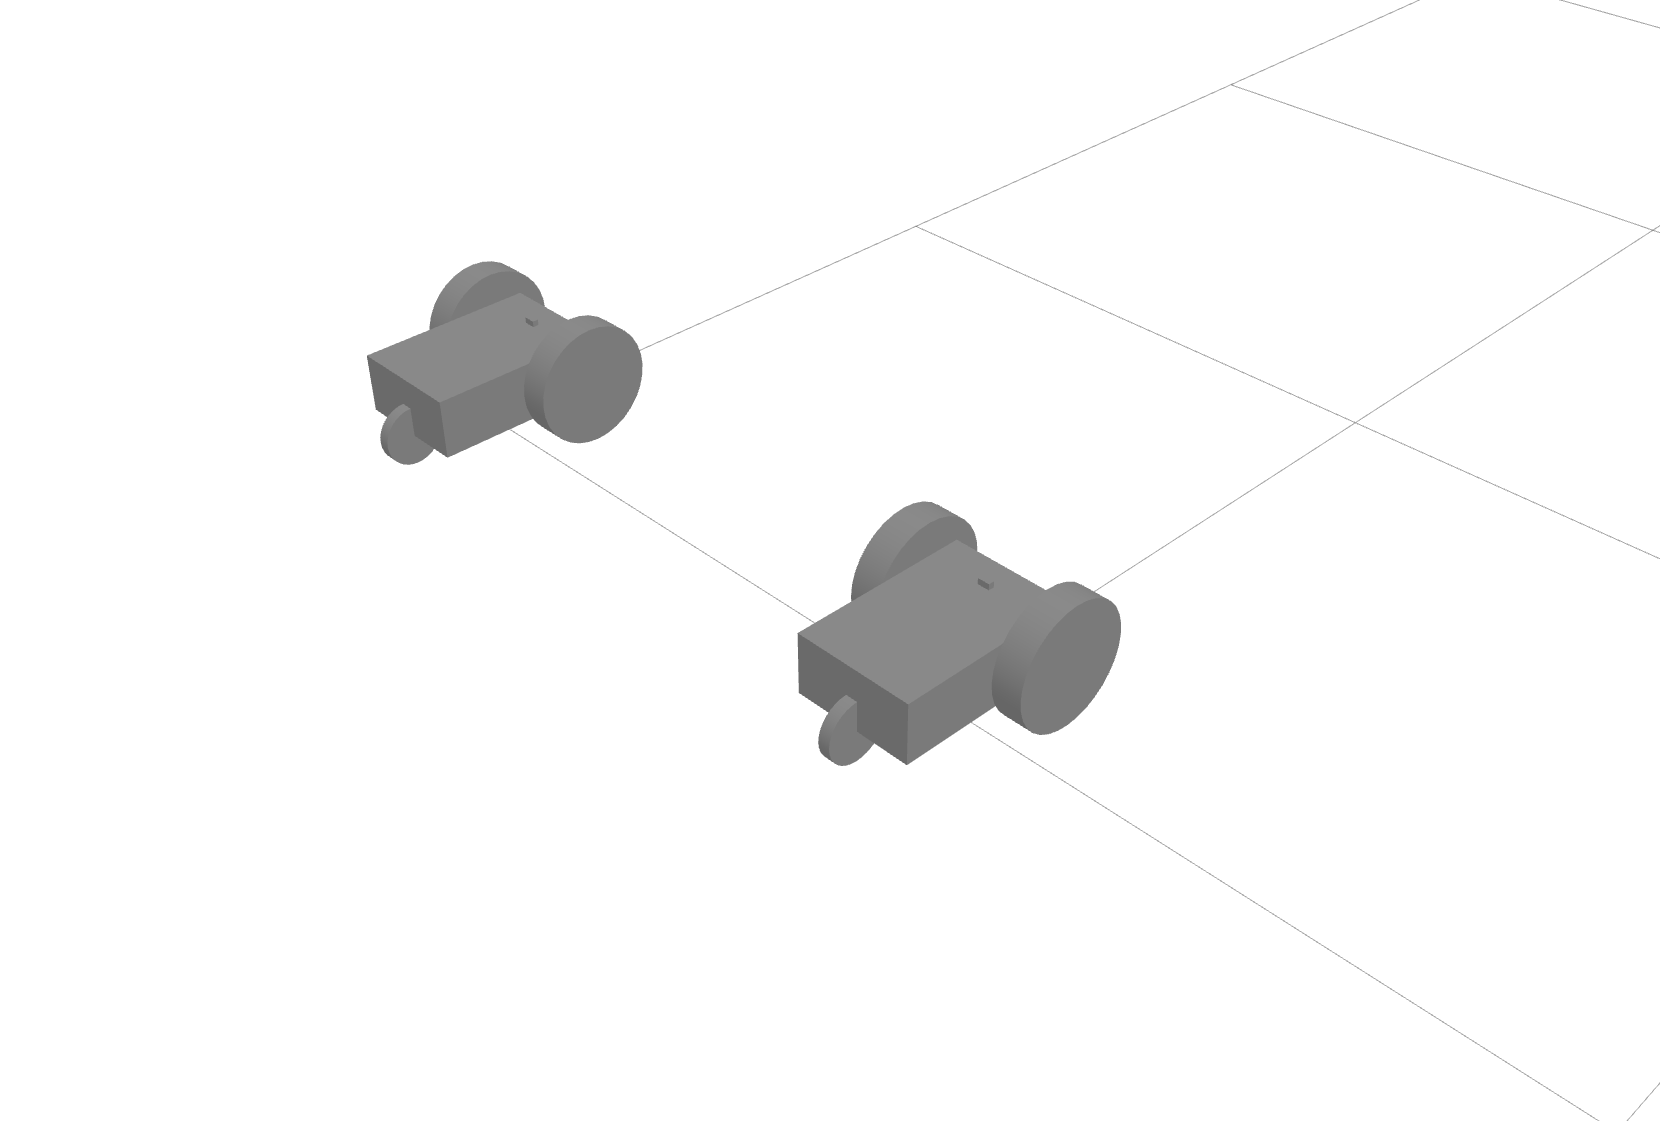
\includegraphics[width=0.5\textwidth]{graphics/crawlers.png}
				\caption{Modèle de crawler utilisé pour l'inspection acoustique de structures métalliques.}
				\label{fig:crawler}
			\end{figure}
		\subsection{Proposition de solution}

			% \begin{Definition}[Proposition (mathématiques)
			% 	\footnote{\url{https://www.techno-science.net/definition/6406.html}, dernière visite le 31/10/2019.}]
			% 	\label{def:troll}
			% 	En mathématiques, dans une théorie donnée, une \textbf{proposition} est un énoncé formé d'un assemblage de symboles et de mots, auquel une valeur de vérité vrai ou faux peut être attribuée, dans certaines conditions mais de la vérité duquel on pourra toujours décider dans toute situation.
			% \end{Definition}

			% Exemple de proposition~:
			% \begin{Proposition}[La Terre sphérique des Anciens\footnote{\url{https://planet-terre.ens-lyon.fr/article/histoire-forme-Terre.xml}, dernière visite le 31/10/2019}]
			% 	\label{prop:f}
			% 	La Terre est supposée plate, de la forme d'un disque, entièrement ceinturée par le fleuve Océan et recouverte d'un ciel en coupole hémi-sphérique.
			% \end{Proposition}
		\subsection{Étude théorique de propriétés de la solution proposée}
			\begin{Theorem}[Théorème de Pythagore]
				\label{Th:Pythagore}
				On nomme $a$, $b$ et $c$ les longueurs des trois côtés d'un triangle.\\
				Les triangles pour lesquels on a la relation $a^{2}+ b^{2} = c^{2}$ sont tous les triangles rectangles dont l'hypoténuse est le côté de longueur $c$, et seulement eux.

				Source : \url{http://mathematiques3.free.fr/2troisieme/problemes/prob014.php}, dernière visite 31/10/2019.
			\end{Theorem}

			On peut aussi écrire des corolaires
			\begin{Corollary}[]
				\label{Cor:TriangleImpossible}
				Il n'existe aucun triangle rectangle ayant les longueurs de côté suivantes~: $3$, $2$ et $23$.
			\end{Corollary}

			Reste à le prouver.
			\begin{proof}
				Pour prouver ce corollaire, procédons par l'absurde en supposant que le triangle soit rectangle. Il y a alors trois possibilités pour la longueur de l'hypoténuse $c$.
				\begin{itemize}
					\item $c=3$\\
					or $2^{2}+ 23^{2} \neq 3^{2}$\\
					donc si le triangle est rectagle, sa longueur ne peut être $3$.
					\item $c=2$\\
					or $3^{2}+ 23^{2} \neq 2^{2}$\\
					donc si le triangle est rectagle, sa longueur ne peut être $2$.
					\item $c=23$\\
					or $2^{2}+ 3^{2} \neq 23^{2}$\\
					donc si le triangle est rectagle, sa longueur ne peut être $23$.
				\end{itemize}
				Donc aucun côté ne satisfait la définition d'une hypoténuse. Le triangle ne peut donc pas être un triangle rectangle.
			\end{proof}
			Il est aussi possible d'écrire des lemmes.

			\begin{Lemma}[Lemme d'Euclide\footnote{\url{https://fr.wikipedia.org/wiki/Lemme_d'Euclide}, dernière visite le 30/10/2019}]
				\label{lem:Euclide}
				Si un nombre premier $p$ divise le produit de deux nombres entiers $b$ et $c$, alors $p$ divise $b$ ou $c$.
			\end{Lemma}
	\section{Implémentations techniques}
		Dans cette section, nous mettons en évidence les différentes implémentations techniques que nous avons développées pour soutenir nos solutions de navigation et de contrôle multi-robots dans le contexte de l'inspection acoustique de structures métalliques.
		Nous commençons par décrire l'algorithme de tracé de sagement de Bresenham, largement utilisé pour déterminer quels sont les points d'un plan discret qui doivent être tracés afin de former une approximation de segment de droite entre deux points donnés.
		Ensuite, nous présentons notre propre implémentation de cet algorithme, qui met à jour notre structure de données localisant les différentes zones de corrosion détectées.
		De plus, nous abordons l'implémentation de l'algorithme de peinture au rouleau, qui permet aux robots de se déplacer de manière synchrone, en suivant des trajectoires parallèles.
		Nous poursuivons avec l'implémentation de l'algorithme du ski nordique, qui permet aux robots de se déplacer de manière asynchrone, en suivant des trajectoires parallèles, modifiant ainsi l'orientation du vecteur représentant la direction de déplacement de l'onde émise et reçue par la paire de robot.
		Ensuite, nous examinons l'implémentation de l'algorithme d'investigation polygonale, qui permt aux robots d'examiner plus précisément des zones suspectes de corrosion.
		Enfin, nous présentons l'algorithme de calcul du $\kappa$ de Cohen, utilisé pour évaluer la qualité et la fiabilité des résultats de l'inspection acoustique. Nous discutons en détail de notre implémentation de cet algorithme, qui fournit des mesures quantitatives pour évaluer la performance des robots dans l'inspection des structures métalliques. Chacune de ces implémentations techniques contribue à l'efficacité et à la précision de notre approche de navigation et de contrôle multi-robots, et sera examinée en détail dans les sous-sections suivantes.
		\subsection*{Algorithme de tracé de segement de Bresenham}
			L'algorithme de tracé de segment de Bresenham est couramment utilisé pour déterminer les points d'un plan discret qui doivent être tracés afin de former une approximation de segment de droite entre deux points donnés.
			Lors du balaiement de la surface à inspecter par une paire de robot émetteur et récepteur, le robot émetteur émet une onde acoustique dans la structure métallique, qui est ensuite reçue par le robot récepteur.
			La détection étant considérée comme parfaite, le robot récepteur reçoit l'onde émise par le robot émetteur, sans quasi altération de la puissance du signal, si et seulement si le segment de droite entre les deux robots ne traverse pas une zone de corrosion.
			Il est ainsi possible de déterminer si une zone de corrosion est présente entre les deux robots en vérifiant si le signal reçu par le robot récepteur est suffisamment puissant.
			Dans la mesure où il n'y a pas de détection de corrosion entre l'émetteur et le récepteur, alors le segment de droite entre les deux robots est considéré comme étant libre de corrosion.
			Dans le cas conraire, alors les points du segment de droite entre les deux robots sont considérés comme étant de la corrosion, à l'exception des points préalablement perçu comme étant libre de corrosion.

			Nous utilisons donc l'algorithme de tracé de segment de Bresenham pour déterminer les points du segment de droite entre les deux robots.
			L'algorithme est présenté à l'algorithme \ref{alg:Bresenham}. La partie adaptée à notre problème se trouve entre les lignes 12 et 17 de ce dernier.
			À cet endroit, nous verrifions si la puissance du signal est suffisamment altérée et si le point du segment de droite entre les deux robots n'a pas déjà été perçu comme étant libre de corrosion.
			Si c'est le cas, alors le point considéré est marqué comme étant de la corrosion, modélisé par la valeur OCCUPIED. Si la puissance du signal n'est pas suffisamment altérée, alors le point considéré est marqué comme étant libre de corrosion, modélisé par la valeur EMPTY.
			Une fois que tous les points du segment ont été parcourus, la grille $G$ est mise à jour avec les nouvelles informations.
			L'algorithme de tracé de segment de Bresenham contribue ainsi à la construction de la grille d'occupation qui permet de localiser les zones de corrosion détectées par les robots lors de l'inspection acoustique des structures métalliques.

			\begin{algorithm}[h!]
				\caption{Process of updating the occupancy grid using Bresenham's line drawing algorithm.}
				\label{alg:Bresenham}
				\KwData{$P_1 \in \mathbb{R}^2$, $P_2 \in \mathbb{R}^2$, $pw \in \mathbb{R}$, $threshold \in \mathbb{R}$, $G$: $l \times w \rightarrow [\text{UNKNOWN}, \text{EMPTY}, \text{OCCUPIED}]$, $l \in \mathbb{N}$, $w \in \mathbb{N}$ \\
					with $P_1$ and $P_2$ the two points to connect, $pw$ the power of the UGW, $threshold$ the threshold above which the power of the UGW is considered undistributed and $G$ the grid to update.}
				\KwResult{The updated grid.}
				$p_0 \gets \text{from\_position\_to\_grid\_coordinate}(P_1)$ \\
				$p_1 \gets \text{from\_position\_to\_grid\_coordinate}(P_2)$ \\
				\If{\text{is\_out\_of\_grid}($p_0$) \textbf{or} \text{is\_out\_of\_grid}($p_1$)}{
					\Return
				}
				$dx \gets p_1.x - p_0.x$ \\
				$dy \gets p_1.y - p_0.y$ \\
				$sx \gets \text{sign}(dx)$ \\
				$sy \gets \text{sign}(dy)$ \\
				$err = dx - dy$ \\
				\While{$p_0 \neq p_1$}{
					\If{$pwd \leq threshold$ \textbf{and} $G(p_0) = \text{UNKNOWN}$}{
						$G(p_0) \gets \text{OCCUPIED}$
					}
					\ElseIf{$pwd > threshold$}{
						$G(p_0) \gets \text{EMPTY}$
					}
					$e2 \gets 2 \times err$ \\
					\If{$e2 > -dy$}{
						$err \gets err - dy$ \\
						$p_0.x \gets p_0.x + sx$
					}
					\If{$e2 < dx$}{
						$err \gets err + dx$ \\
						$p_0.y \gets p_0.y + sy$
					}
				}
			\end{algorithm}
		\subsection*{Algorithme de peinture au rouleau}
			Nous présentons dans cette sous-section l'implémentation de l'algorithme de peinture au rouleau, présenté au listing~\ref{lst:peinture_au_rouleau}.

			\TODO{Implémentation algorithme peinture au rouleu}
		\subsection*{Algorithme de ski nordique}
			Nous présentons dans cette sous-section l'implémentation de l'algorithme de ski nordique, présenté au listing~\ref{lst:ski_nordique}.

			\TODO{Implémentation algorithme ski nordique}
		\subsection*{Algorithme d'investigation polygonale}
			Nous présentons dans cette sous-section l'implémentation de l'algorithme d'investigation polygonale, présenté au listing~\ref{lst:investigation_polygonale}.

			\TODO{Implémentation algorithme investigation polygonale}
		\subsection*{Algorithme de calcul du $\kappa$ de Cohen}
			L'évaluation de la qualité et de la fiabilité des résultats de l'inspection acoustique est essentielle pour garantir des mesures précises de l'état des structures métalliques.
			Dans cette sous-section, nous présentons l'algorithme du calcul du $\kappa$ de Cohen, présenté à l'algorithme \ref{alg:Cohen_Kappa}, une mesure statistique couramment utilisée pour évaluer l'accord entre les résultats obtenus par les robots et une référence humaine.

			L'algorithme de calcul du $\kappa$ de Cohen se base sur la notion de concordance et de discordance entre les résultats des inspections réalisées par les robots et celles réalisées par des inspecteurs humains.
			Il prend en compte les résultats positifs, négatifs, faux positifs et faux négatifs obtenus lors de l'inspection acoustique.
			Ces informations sont utilisées pour calculer la valeur du coefficient de Cohen, noté $\kappa$, avec $\kappa = \frac{p_o - p_e}{1 - p_e}$, où $p_o$ est le taux d'accord observé et $p_e$ le taux d'accord attendu.

			L'algorithme se déroule en plusieurs étapes.
			Tout d'abord, les résultats des inspections réalisées par les robots et réel répartition des zones de corrosion sont comparés pour chaque zone inspectée.
			Ensuite, les résultats sont regroupés en quatre catégories : concordance positive, concordance négative, discordance positive (faux positifs) et discordance négative (faux négatifs).
			Ces catégories sont utilisées pour calculer les taux d'observation et d'accord observés entre les robots et la véritable répartition des zones de corrosion.
			Le $\kappa$ de Cohen est ensuite calculé à partir des taux d'observation et d'accord observés, prenant en compte la possibilité de concordance due au hasard.
			Plus le $\kappa$ de Cohen se rapproche de 1, plus il y a un accord élevé entre les résultats des robots et ceux des inspecteurs humains.
			En revanche, un $\kappa$ proche de 0 indique un faible niveau d'accord, tandis qu'un $\kappa$ négatif suggère une discordance entre les résultats.

			Nous avons implémenté cet algorithme dans le cadre de notre projet, en utilisant les résultats des inspections acoustiques effectuées par les robots et des cartes composées de zones de corrosion comme base de comparaison.
			Cette implémentation nous permet d'obtenir des mesures quantitatives pour évaluer la performance de notre approche de navigation et de contrôle multi-robots dans l'inspection des structures métalliques.
			Dans les prochaines sections, nous détaillerons les résultats obtenus grâce à l'application de cet algorithme du calcul du $\kappa$ de Cohen.

			\begin{algorithm}[h!]
				\caption{Cohen's kappa Algorithm.}
				\label{alg:Cohen_Kappa}
				\KwData{$I_0$: $l \times w \times 3 \rightarrow [0 .. 255]$, $I$: $l \times w \times 3 \rightarrow [0 .. 255]$, $l \in \mathbb{N}$, $w \in \mathbb{N}$ \\
					with $I_0$ the ground truth image and $I$ the image to score.}
				\KwResult{$\kappa \in [0, 1]$}
				$TP \gets 0$ \\
				$TN \gets 0$ \\
				$FP \gets 0$ \\
				$FN \gets 0$ \\
				\For{$i \gets 1$ \KwTo $l$}{
					\For{$j \gets 1$ \KwTo $w$}{
						\If{$\text{is\_label\_1}(I_0(i, j))$}{
							\If{$\text{is\_label\_1}(I(i, j))$}{
								$TP \gets TP + 1$
							}
							\Else{
								$FN \gets FN + 1$
							}
						}
						\Else{
							\If{$\text{is\_label\_1}(I(i, j))$}{
								$FP \gets FP + 1$
							}
							\Else{
								$TN \gets TN + 1$
							}
						}
					}
				}
				$f_c \gets \frac{(TN + FN) (TN + FP) + (FP + TP) (FN + TP)}{TP + TN + FN +FP}$ \\
				$\kappa \gets \frac{TP + TN - f_c}{TP + TN + FN + FP - f_c}$
			\end{algorithm}
	\section{Expérimentations, validations et évaluations}
		\begin{figure}[h!]
			\begin{subfigure}[t]{0.3\linewidth}
				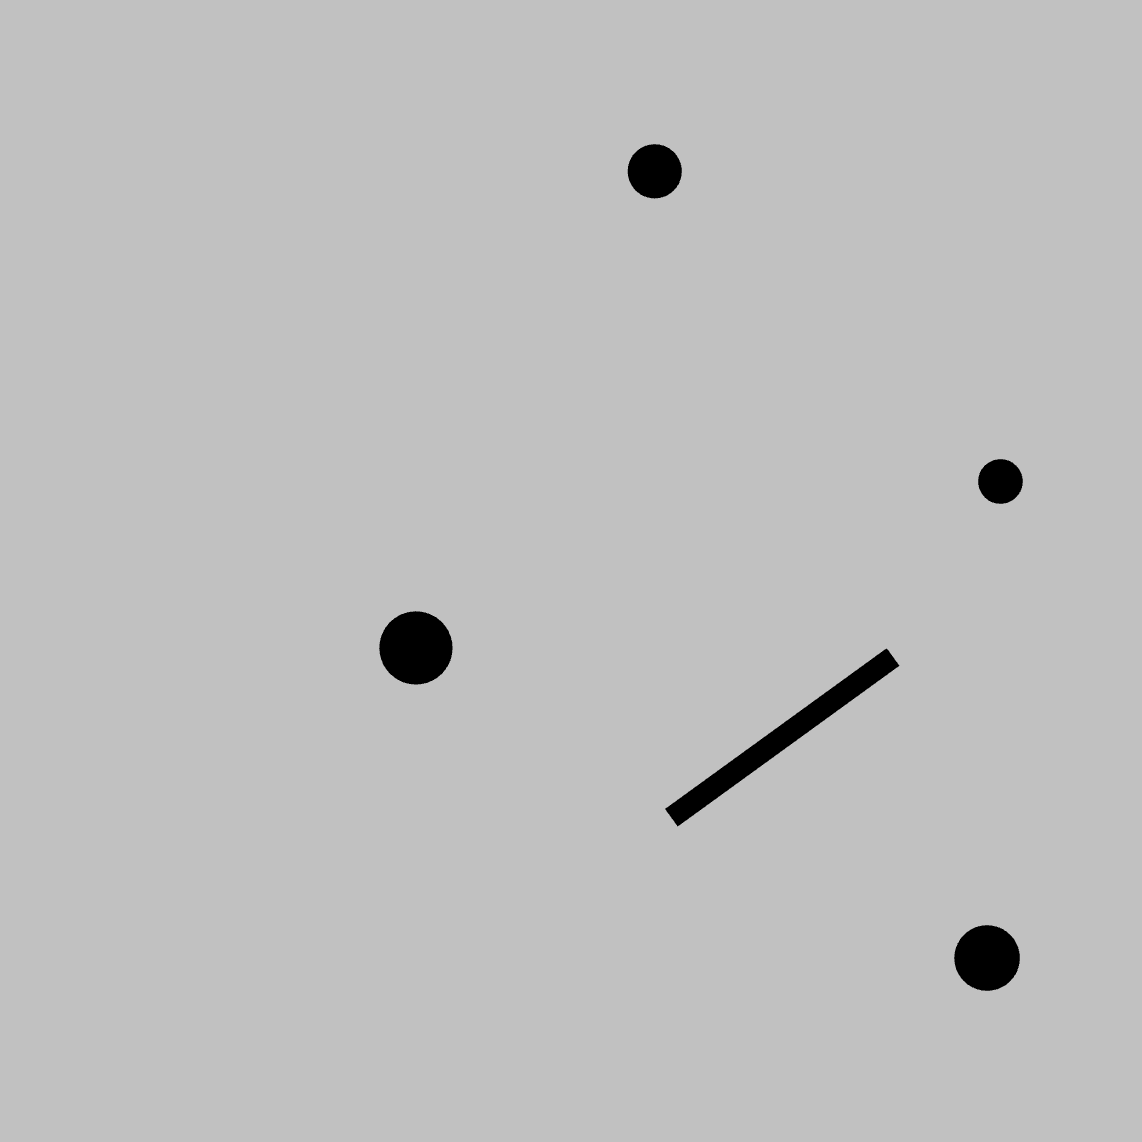
\includegraphics[width=\linewidth]{graphics/test_model_5.png}
				\caption{Test model 5 (density = 1.29\%)}
				\label{fig:test_model_5}
			\end{subfigure}
			\hfill
			\begin{subfigure}[t]{0.3\linewidth}
					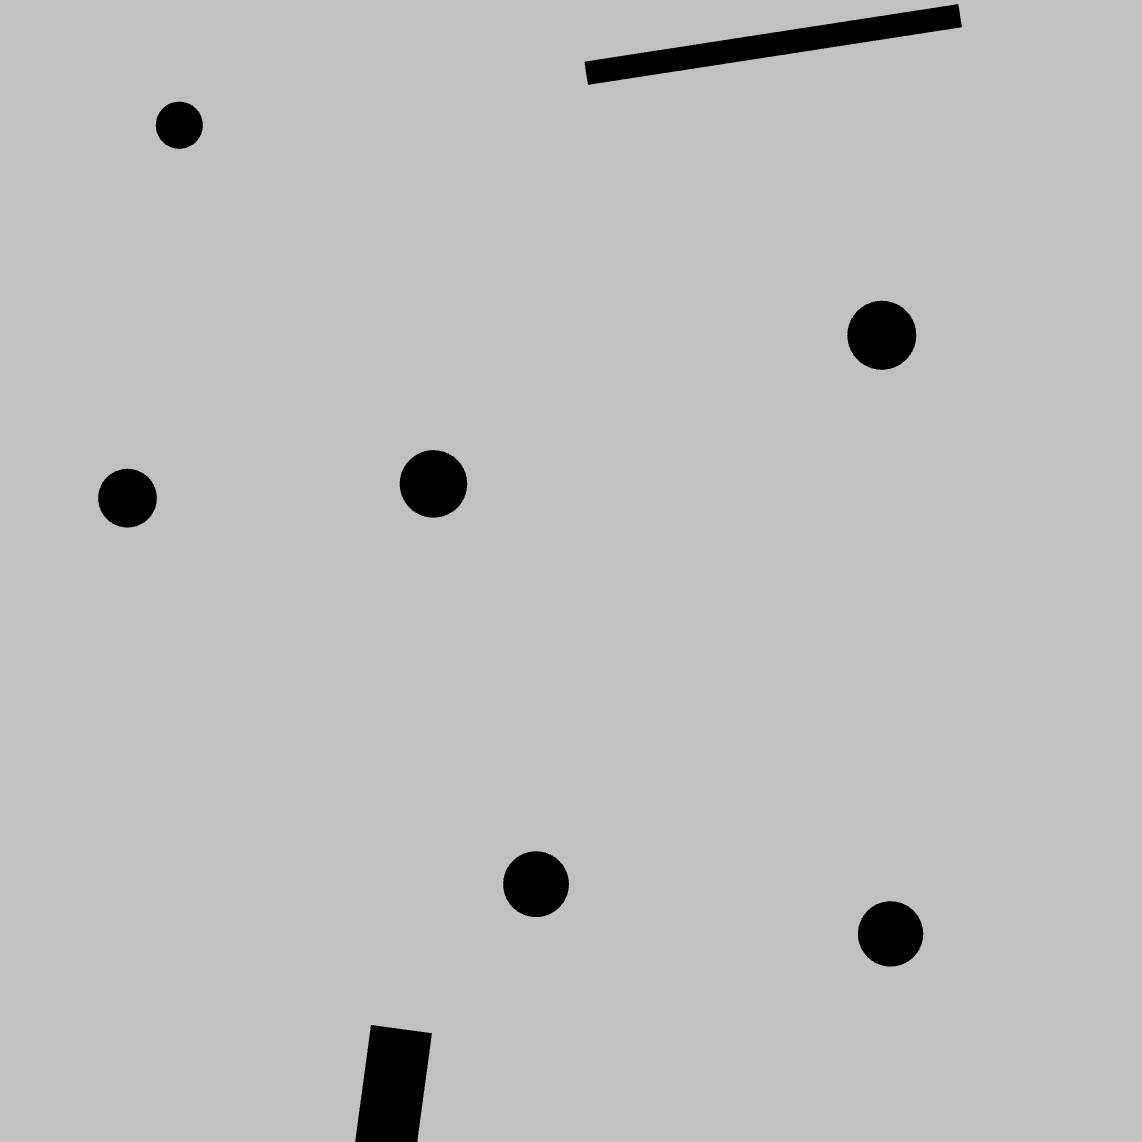
\includegraphics[width=\linewidth]{graphics/test_model_8.png}
					\caption{Test model 8 (density = 2.26\%)}
					\label{fig:test_model_8}
			\end{subfigure}
			\hfill
			\begin{subfigure}[t]{0.3\linewidth}
					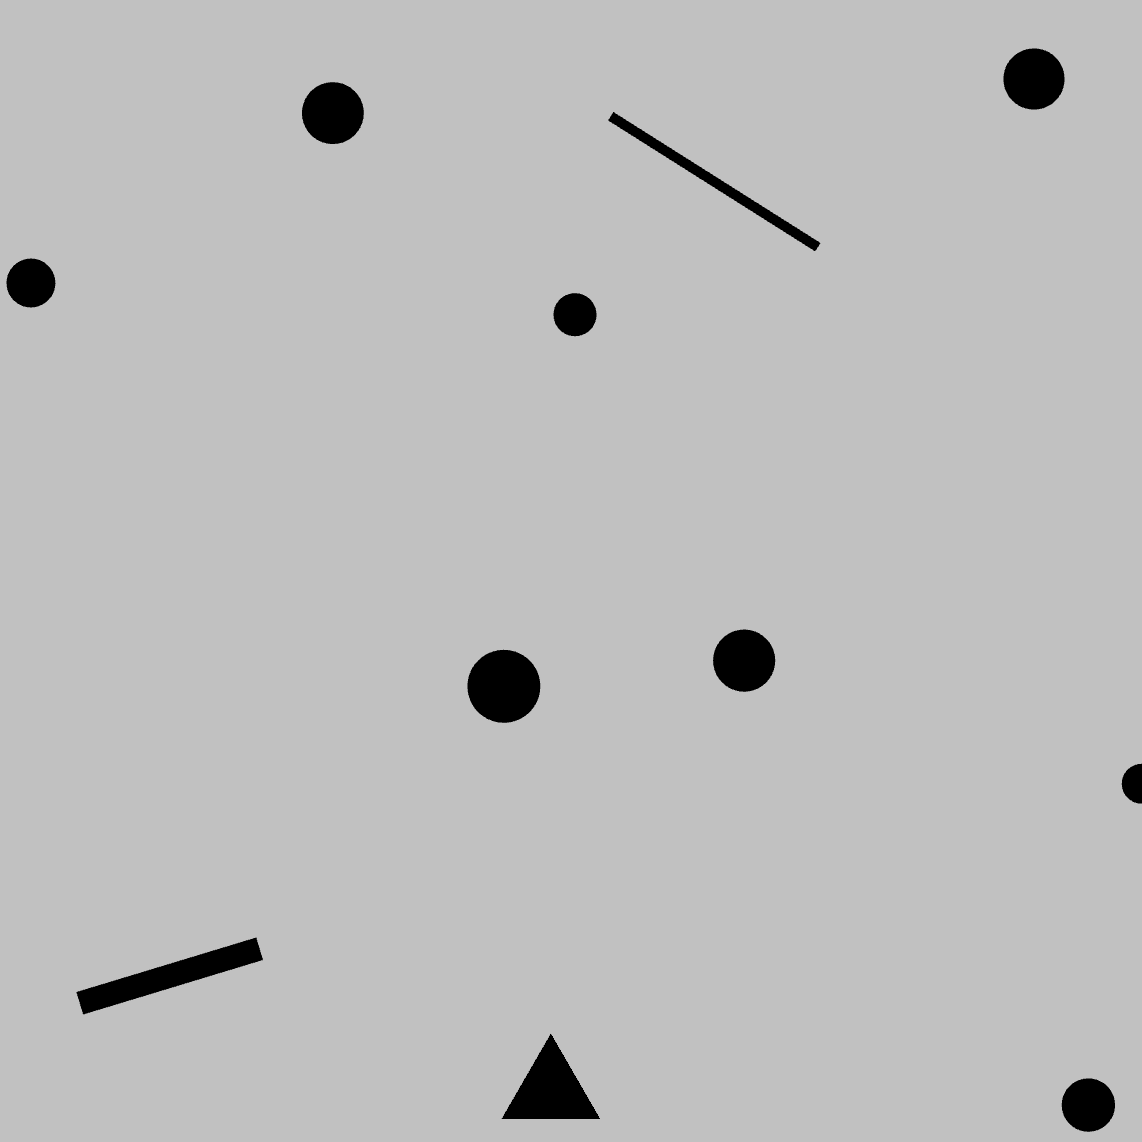
\includegraphics[width=\linewidth]{graphics/test_model_11.png}
					\caption{Test model 11 (density = 2.23\%)}
					\label{fig:test_model_11}
			\end{subfigure}
			\hfill
			\begin{subfigure}[t]{0.3\linewidth}
					
\includegraphics[width=\linewidth]{graphics/test_model_15.png}
					\caption{Test model 15 (density = 2.25\%)}
					\label{fig:test_model_15}
			\end{subfigure}
			\hfill
			\begin{subfigure}[t]{0.3\linewidth}
					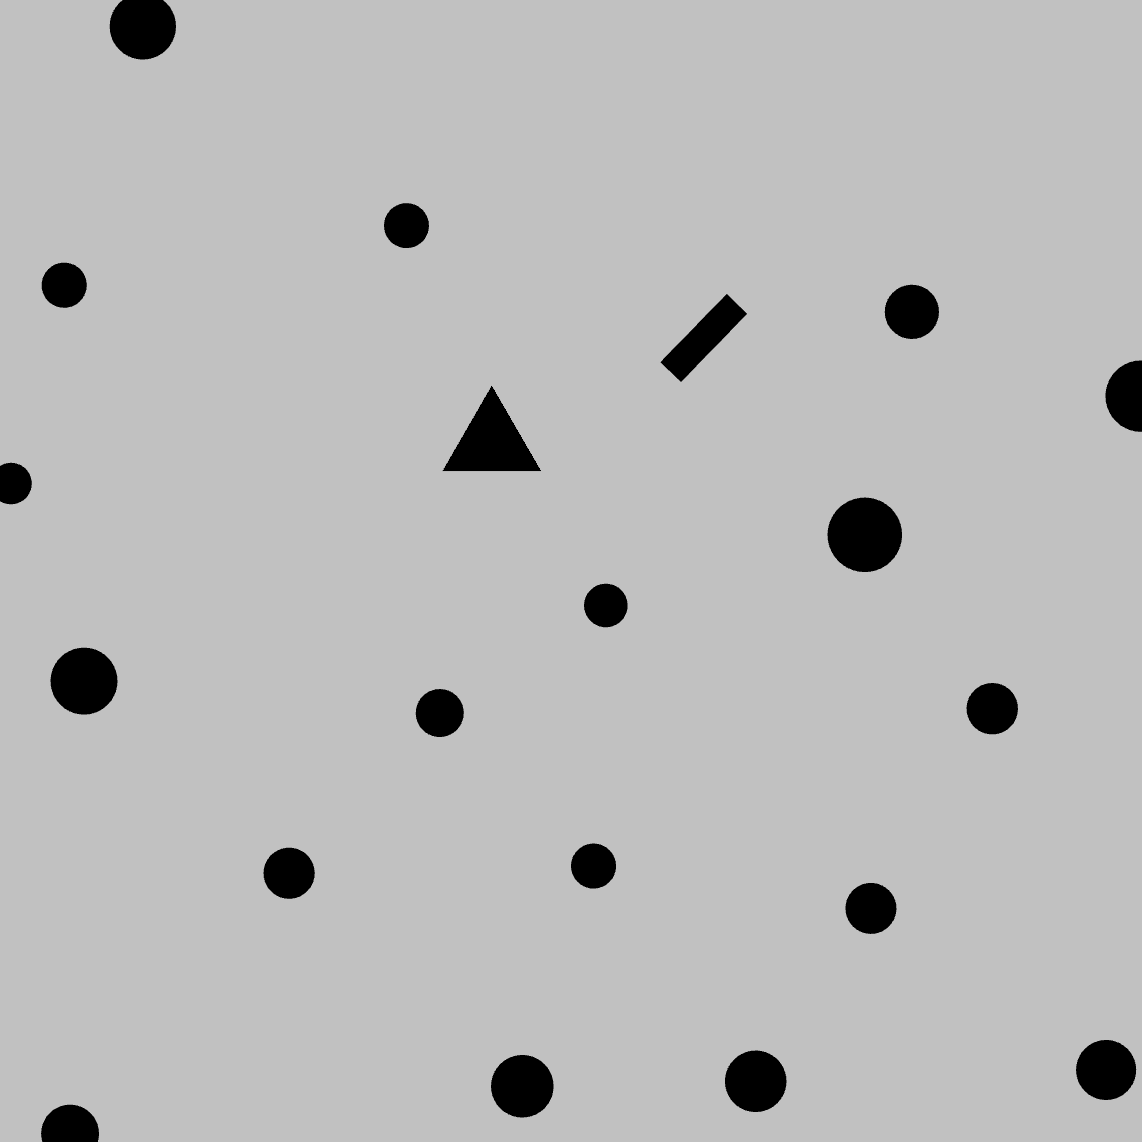
\includegraphics[width=\linewidth]{graphics/test_model_20.png}
					\caption{Test model 20 (density = 3.62\%)}
					\label{fig:test_model_20}
			\end{subfigure}
			\hfill
			\begin{subfigure}[t]{0.3\linewidth}
					
\includegraphics[width=\linewidth]{graphics/test_model_30.png}
					\caption{Test model 30 (density = 5.23\%)}
					\label{fig:test_model_30}
			\end{subfigure}
			\hfill
			\begin{subfigure}[t]{0.3\linewidth}
					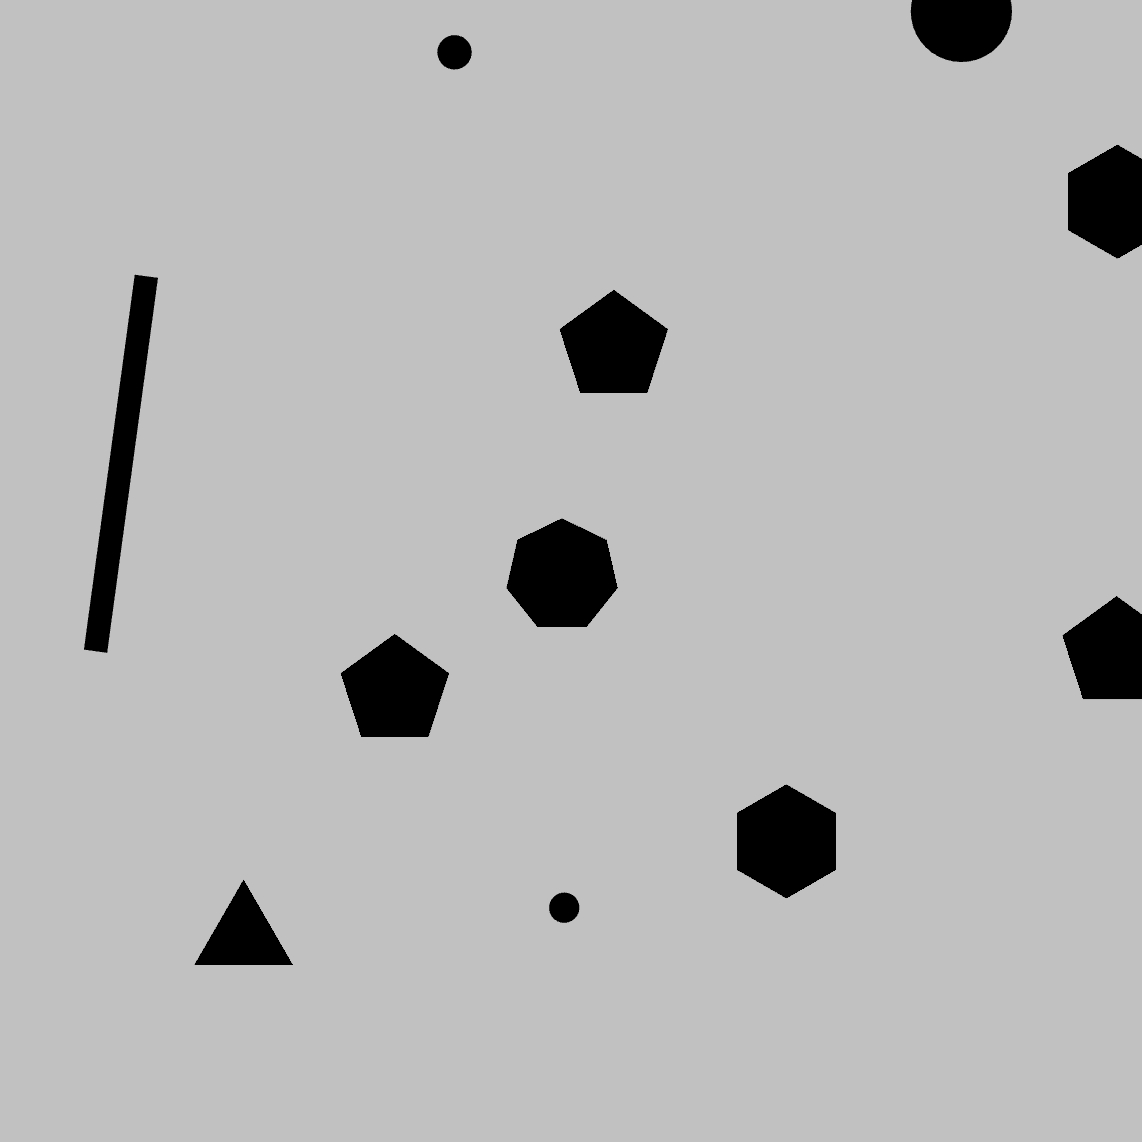
\includegraphics[width=\linewidth]{graphics/test_model_11_complex.png}
					\caption{Test model 11 complex (density = 4.99\%)}
					\label{fig:test_model_11_complex}
			\end{subfigure}
			\hfill
			\begin{subfigure}[t]{0.3\linewidth}
					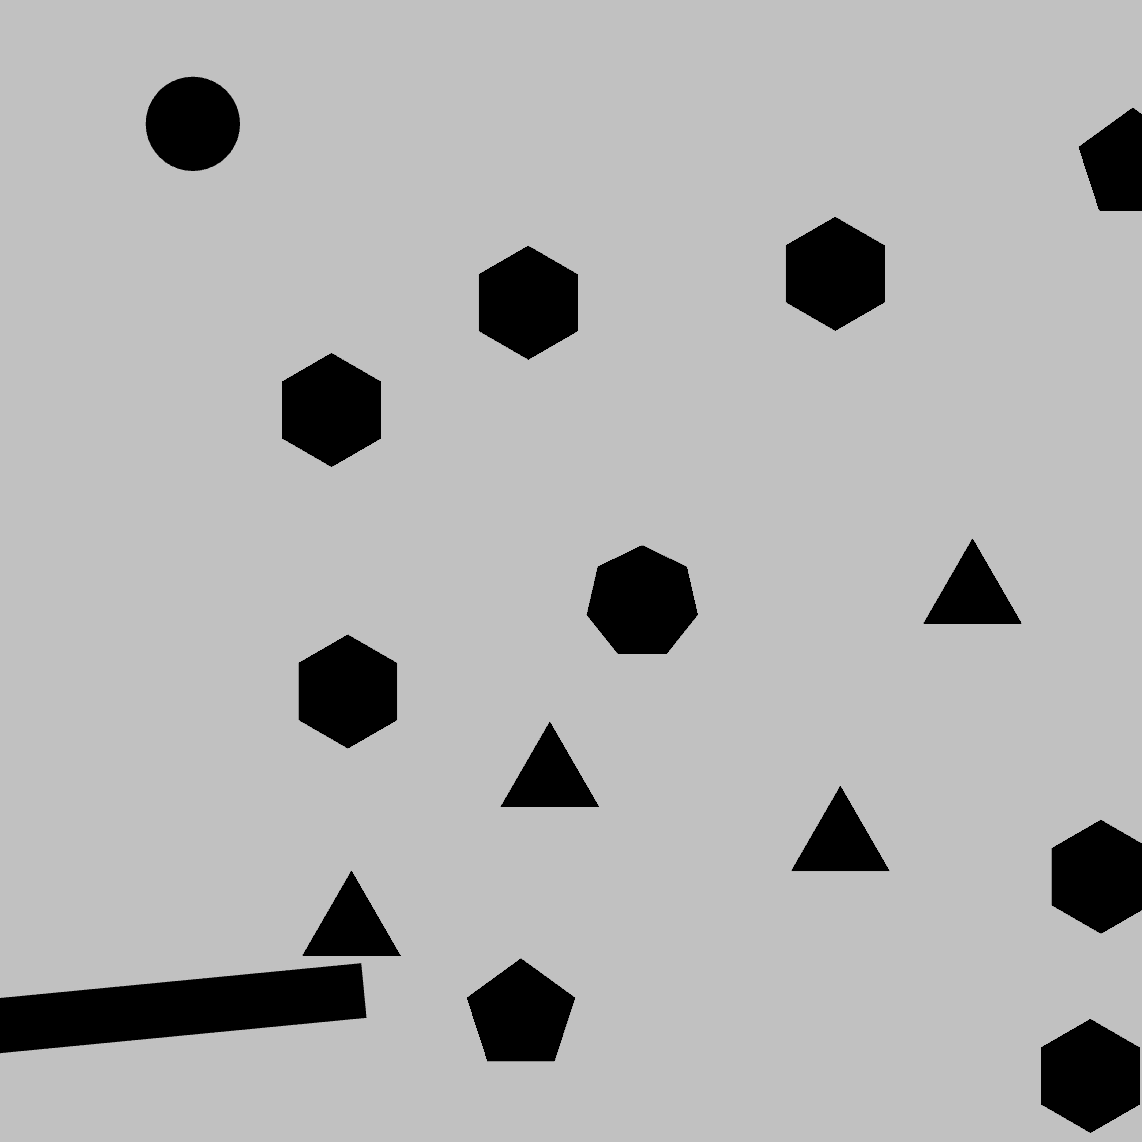
\includegraphics[width=\linewidth]{graphics/test_model_15_complex.png}
					\caption{Test model 15 complex (density = 8.81\%)}
					\label{fig:test_model_15_complex}
			\end{subfigure}
			\caption{Différents environnements de test.}
			\label{fig:test_models}
		\end{figure}

		\begin{figure}[h!]
			\begin{subfigure}[t]{0.49\linewidth}
				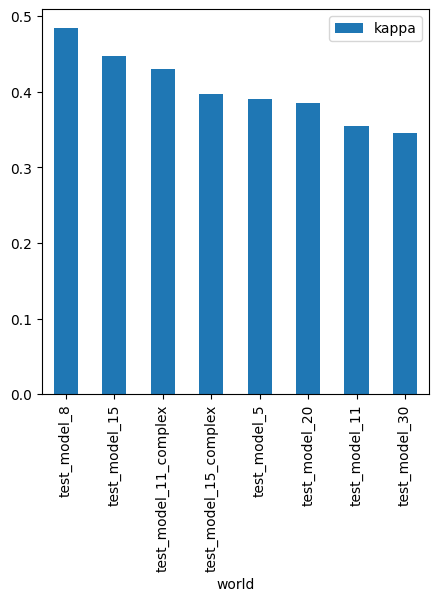
\includegraphics[width=\linewidth]{graphics/peinture_au_rouleau-kappa_vs_world.png}
				\caption{Cohen's kappa vs. world density}
				\label{fig:peinture_au_rouleau-kappa_vs_world}
			\end{subfigure}
			\hfill
			\begin{subfigure}[t]{0.49\linewidth}
					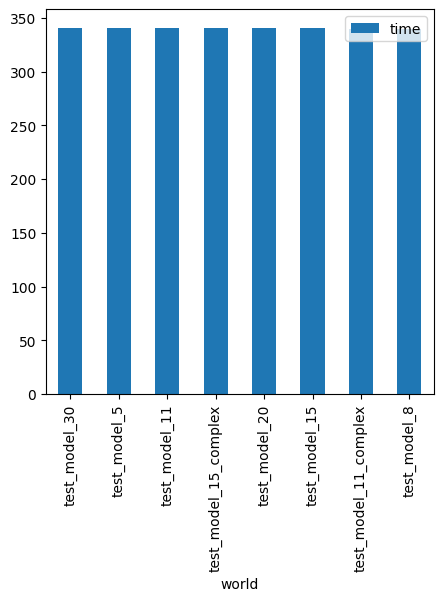
\includegraphics[width=\linewidth]{graphics/peinture_au_rouleau-time_vs_world.png}
					\caption{Time vs. world density}
					\label{fig:peinture_au_rouleau-time_vs_world}
			\end{subfigure}
			\caption{Évolution du score de Cohen et du temps d'exécution de l'algorithme de peinture au rouleau en fonction de la densité du monde.}
			\label{fig:peinture_au_rouleau-world}
		\end{figure}

		\begin{figure}[h!]
			\begin{subfigure}[t]{0.49\linewidth}
				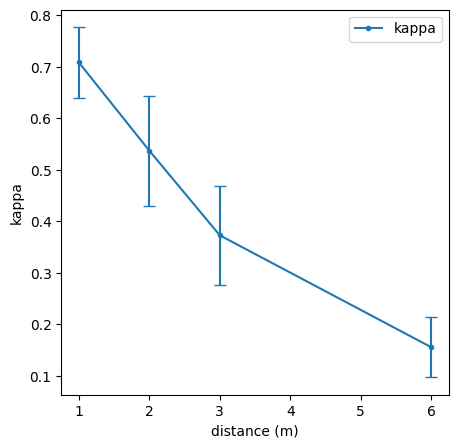
\includegraphics[width=\linewidth]{graphics/peinture_au_rouleau-kappa_vs_distance.png}
				\caption{Cohen's kappa vs. crawlers distance}
				\label{fig:peinture_au_rouleau-kappa_vs_distance}
			\end{subfigure}
			\hfill
			\begin{subfigure}[t]{0.49\linewidth}
					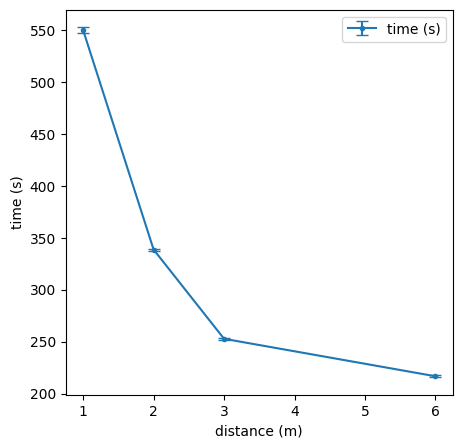
\includegraphics[width=\linewidth]{graphics/peinture_au_rouleau-time_vs_distance.png}
					\caption{Time vs. crawlers distance}
					\label{fig:peinture_au_rouleau-time_vs_distance}
			\end{subfigure}
			\caption{Évolution du score de Cohen et du temps d'exécution de l'algorithme de peinture au rouleau en fonction de la distance qui sépare les deux crawlers.}
			\label{fig:peinture_au_rouleau-distance}
		\end{figure}

		\begin{figure}[h!]
			\begin{subfigure}[t]{0.49\linewidth}
				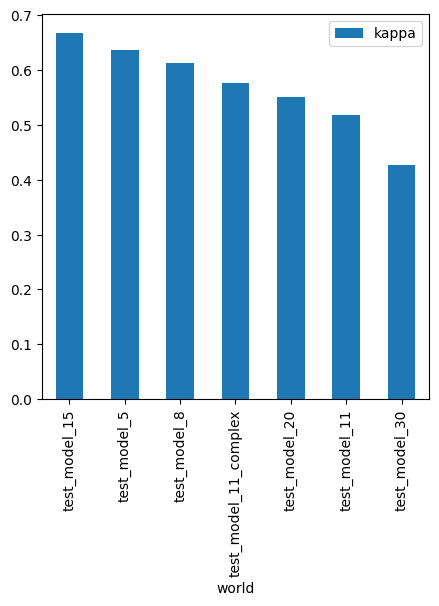
\includegraphics[width=\linewidth]{graphics/ski_nordique-kappa_vs_world.png}
				\caption{Cohen's kappa vs. world density}
				\label{fig:ski_nordique-kappa_vs_world}
			\end{subfigure}
			\hfill
			\begin{subfigure}[t]{0.49\linewidth}
					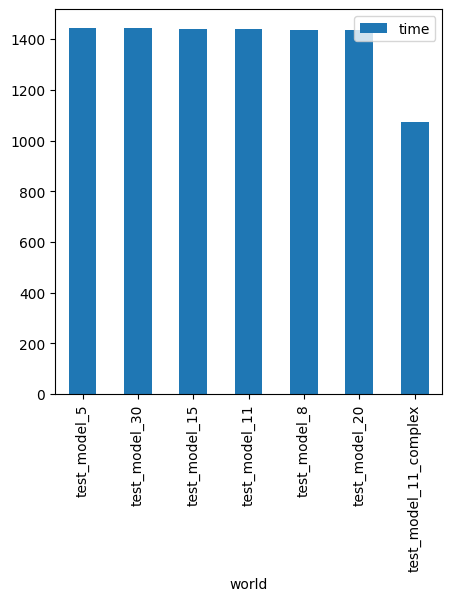
\includegraphics[width=\linewidth]{graphics/ski_nordique-time_vs_world.png}
					\caption{Time vs. world density}
					\label{fig:ski_nordique-time_vs_world}
			\end{subfigure}
			\caption{Évolution du score de Cohen et du temps d'exécution de l'algorithme de ski nordique en fonction de la densité du monde.}
			\label{fig:ski_nordique-world}
		\end{figure}

		\begin{figure}[h!]
			\begin{subfigure}[t]{0.49\linewidth}
				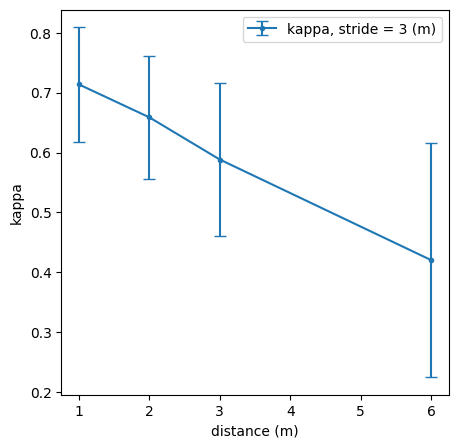
\includegraphics[width=\linewidth]{graphics/ski_nordique-kappa_vs_distance.png}
				\caption{Cohen's kappa vs. crawlers distance}
				\label{fig:ski_nordique-kappa_vs_distance}
			\end{subfigure}
			\hfill
			\begin{subfigure}[t]{0.49\linewidth}
					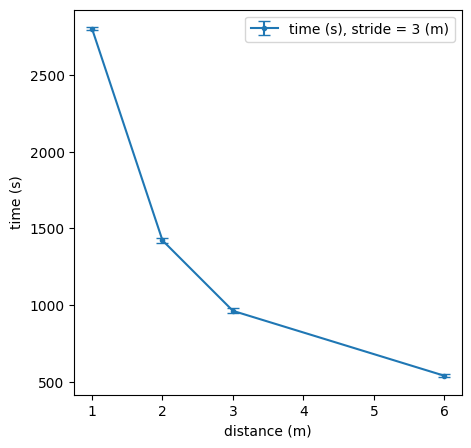
\includegraphics[width=\linewidth]{graphics/ski_nordique-time_vs_distance.png}
					\caption{Time vs. crawlers distance}
					\label{fig:ski_nordique-time_vs_distance}
			\end{subfigure}
			\caption{Évolution du score de Cohen et du temps d'exécution de l'algorithme de ski nordique en fonction de la distance qui sépare les deux crawlers.}
			\label{fig:ski_nordique-distance}
		\end{figure}

		\begin{figure}[h!]
			\begin{subfigure}[t]{0.49\linewidth}
				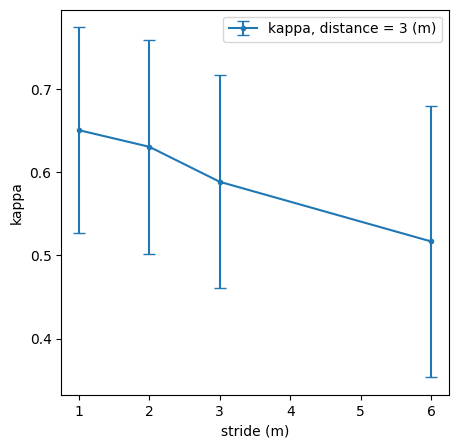
\includegraphics[width=\linewidth]{graphics/ski_nordique-kappa_vs_stride.png}
				\caption{Cohen's kappa vs. crawlers stride}
				\label{fig:ski_nordique-kappa_vs_stride}
			\end{subfigure}
			\hfill
			\begin{subfigure}[t]{0.49\linewidth}
					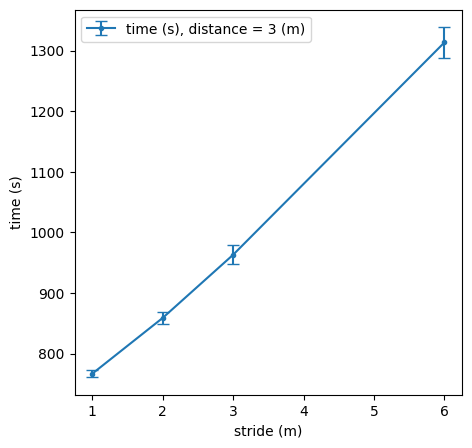
\includegraphics[width=\linewidth]{graphics/ski_nordique-time_vs_stride.png}
					\caption{Time vs. crawlers stride}
					\label{fig:ski_nordique-time_vs_stride}
			\end{subfigure}
			\caption{Évolution du score de Cohen et du temps d'exécution de l'algorithme de ski nordique en fonction de la foulée qui sépare les deux crawlers.}
			\label{fig:ski_nordique-stride}
		\end{figure}

		\begin{figure}[h!]
			\begin{subfigure}[t]{0.49\linewidth}
				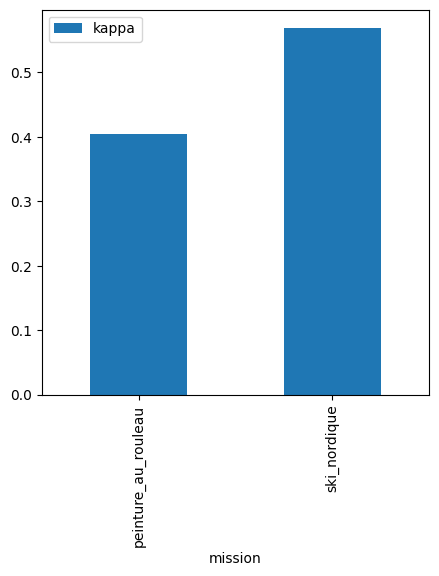
\includegraphics[width=\linewidth]{graphics/peinture_au_rouleau-kappa_vs_ski_nordique-kappa.png}
				\caption{Roller painting Cohen's kappa vs. Nordic skiing Cohen's kappa}
				\label{fig:peinture_au_rouleau-kappa_vs_ski_nordique-kappa}
			\end{subfigure}
			\hfill
			\begin{subfigure}[t]{0.49\linewidth}
					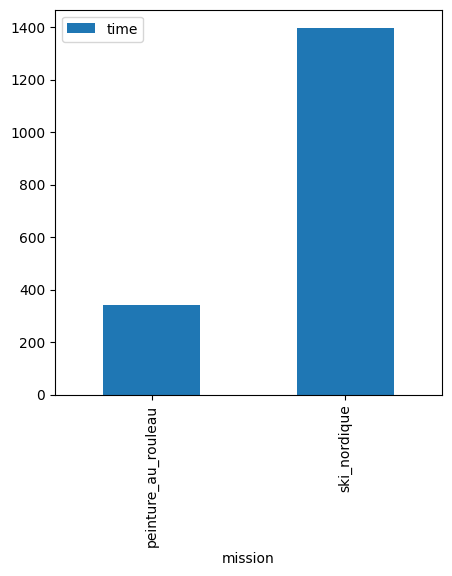
\includegraphics[width=\linewidth]{graphics/peinture_au_rouleau-time_vs_ski_nordique-time.png}
					\caption{Roller painting time vs. Nordic skiing time}
					\label{fig:peinture_au_rouleau-time_vs_ski_nordique-time}
			\end{subfigure}
			\caption{Score de Cohen et temps d'exécution des algorithmes de peinture au rouleau et de ski nordique.}
			\label{fig:peinture_au_rouleau_vs_ski_nordique}
		\end{figure}
	\section{Bilan personnel}
		\TODO{Bilan personnel}
	\section{Conclusion et perspectives}
		\TODO{Conclusion et perspectives}
	\section*{}
	\bibliographystyle{unsrt}
	\bibliography{rapportPFE}
	\appendix
	\section{Implémentation de l'algorithme de peinture au rouleau}
		\begin{lstlisting}[language=Python,caption={Implémentation de l'algorithme de peinture au rouleau},label=lst:peinture_au_rouleau]
#!/usr/bin/env python3
import rospy
import numpy
from math import *
from task_manager_lib.TaskClient import *

rospy.init_node('task_client')
server_node = rospy.get_param("~server", "/crawler_id/task_server")
default_period = rospy.get_param("~period", 0.05)
tc = TaskClient(server_node, default_period)
rospy.loginfo("Mission connected to server: " + server_node)
vel = rospy.get_param("~velocity", 0.5)
crawler_id = rospy.get_param("~crawler_id", 0)
crawlers_distance = rospy.get_param("~crawlers_distance", 1.0)
overlap = rospy.get_param("~overlap", 0.1)
width = rospy.get_param("~width", 20.0)
height = rospy.get_param("~height", 20.0)

d = crawlers_distance
k = 0
stat = 0

start = rospy.Time.now()

try:
	tc.SetStatusSync(status=stat)
	if crawler_id == 0:
		tc.WaitForStatusSync(partner="crawler_1", status=stat)
	elif crawler_id == 1:
		tc.WaitForStatusSync(partner="crawler_0", status=stat)
	stat += 1

	# vertical
	if crawler_id == 0:
		for i in numpy.arange(-width/2, width/2-d+1, d):
			tc.AlignWithTarget(goal_x=i-overlap, goal_y=height/2*(-1)**k)
			tc.FollowLine(goal_x=i-overlap, goal_y=height/2*(-1)**k, max_velocity=vel)
			tc.AlignWithTarget(goal_x=i+d-overlap, goal_y=height/2*(-1)**k)
			tc.FollowLine(goal_x=i+d-overlap, goal_y=height/2*(-1)**k, max_velocity=vel)
			k = (k+1) % 2
			tc.SetStatusSync(status=stat)
			tc.WaitForStatusSync(partner="crawler_1", status=stat)
			stat += 1
	elif crawler_id == 1:
		for i in numpy.arange(-width/2+d, width/2+1, d):
			tc.AlignWithTarget(goal_x=i+overlap, goal_y=height/2*(-1)**k)
			tc.FollowLine(goal_x=i+overlap, goal_y=height/2*(-1)**k, max_velocity=vel)
			tc.AlignWithTarget(goal_x=i+d+overlap, goal_y=height/2*(-1)**k)
			tc.FollowLine(goal_x=i+d+overlap, goal_y=height/2*(-1)**k, max_velocity=vel)
			k = (k+1) % 2
			tc.SetStatusSync(status=stat)
			tc.WaitForStatusSync(partner="crawler_0", status=stat)
			stat += 1

	if crawler_id == 0:
		tc.GoTo(goal_x=width/2+d, goal_y=-height/2, max_velocity=vel)
		tc.SetStatusSync(status=stat)
		tc.WaitForStatusSync(partner="crawler_1", status=stat)
		stat += 1
		tc.GoTo(goal_x=width/2, goal_y=-height/2, max_velocity=vel)
		tc.SetStatusSync(status=stat)
		tc.WaitForStatusSync(partner="crawler_1", status=stat)
	elif crawler_id == 1:
		tc.GoTo(goal_x=width/2+d, goal_y=-height/2+d, max_velocity=vel)
		tc.SetStatusSync(status=stat)
		tc.WaitForStatusSync(partner="crawler_0", status=stat)
		stat += 1
		tc.GoTo(goal_x=width/2, goal_y=-height/2+d, max_velocity=vel)
		tc.SetStatusSync(status=stat)
		tc.WaitForStatusSync(partner="crawler_0", status=stat)
	stat += 1
	k = 1

	# horizontal
	if crawler_id == 0:
		for i in numpy.arange(-height/2, height/2-d+1, d):
			tc.AlignWithTarget(goal_x=width/2*(-1)**k, goal_y=i-overlap)
			tc.FollowLine(goal_x=width/2*(-1)**k, goal_y=i-overlap, max_velocity=vel)
			tc.AlignWithTarget(goal_x=width/2*(-1)**k, goal_y=i+d-overlap)
			tc.FollowLine(goal_x=width/2*(-1)**k, goal_y=i+d-overlap, max_velocity=vel)
			k = (k+1) % 2
			tc.SetStatusSync(status=stat)
			tc.WaitForStatusSync(partner="crawler_1", status=stat)
			stat += 1
	elif crawler_id == 1:
		for i in numpy.arange(-height/2+d, height/2+1, d):
			tc.AlignWithTarget(goal_x=width/2*(-1)**k, goal_y=i+overlap)
			tc.FollowLine(goal_x=width/2*(-1)**k, goal_y=i+overlap, max_velocity=vel)
			tc.AlignWithTarget(goal_x=width/2*(-1)**k, goal_y=i+d+overlap)
			tc.FollowLine(goal_x=width/2*(-1)**k, goal_y=i+d+overlap, max_velocity=vel)
			k = (k+1) % 2
			tc.SetStatusSync(status=stat)
			tc.WaitForStatusSync(partner="crawler_0", status=stat)
			stat += 1

except TaskException as e:
	rospy.logerr("Exception caught: " + str(e))

end = rospy.Time.now()
time = (end-start).to_sec()
rospy.loginfo("Mission completed in " + str(time) + " seconds")
		\end{lstlisting}
	\section{Implémentation de l'algorithme de ski nordique}
		\begin{lstlisting}[language=Python,caption={Implémentation de l'algorithme de ski nordique},label=lst:ski_nordique]
#!/usr/bin/env python3
from time import sleep
import rospy
import numpy
from math import *
from task_manager_lib.TaskClient import *

rospy.init_node('task_client')
server_node = rospy.get_param("~server", "/crawler_id/task_server")
default_period = rospy.get_param("~period", 0.05)
tc = TaskClient(server_node, default_period)
rospy.loginfo("Mission connected to server: " + server_node)
vel = rospy.get_param("~velocity", 0.5)
crawler_id = rospy.get_param("~crawler_id", 0)
crawlers_distance = rospy.get_param("~crawlers_distance", 1.0)
stride_size = int(rospy.get_param("~stride_size", 1.0))
overlap = rospy.get_param("~overlap", 0.1)
grid_width = rospy.get_param("~grid_width", 6) // 2
grid_height = rospy.get_param("~grid_height", 6) // 2

d = crawlers_distance
k = 0
if crawler_id == 0: overlap = -overlap

start = rospy.Time.now()

# vertical pass

if crawler_id == 0: begin_w, end_w = -grid_width, grid_width + 1 - d
elif crawler_id == 1: begin_w, end_w = -grid_width + d, grid_width + 1

stat = 0
tc.SetStatusSync(status=stat)
if crawler_id == 0: tc.WaitForStatusSync(partner="crawler_1", status=stat+1)

for i in numpy.arange(begin_w, end_w, d):

	if crawler_id == 0: begin_h, end_h = -grid_height + 2*stride_size, grid_height + 1 + stride_size
	elif crawler_id == 1: begin_h, end_h = -grid_height + stride_size, grid_height + 1 + stride_size

	for j in numpy.arange(begin_h, end_h, 2*stride_size):
		tc.GoTo(goal_x=i+overlap, goal_y=j, max_velocity=vel, relative=False)
		stat += 1
		tc.SetStatusSync(status=stat)
		if crawler_id == 0: tc.WaitForStatusSync(partner="crawler_1", status=stat+1)
		elif crawler_id == 1: tc.WaitForStatusSync(partner="crawler_0", status=stat)

	tc.SetStatusSync(status=stat+1)
	if stride_size % 2 == 1:
		if crawler_id == 0: tc.GoTo(goal_x=i+overlap, goal_y=grid_height + stride_size, max_velocity=vel, relative=False)
		if crawler_id == 1: tc.GoTo(goal_x=i+overlap, goal_y=grid_height, max_velocity=vel, relative=False)
	elif stride_size % 2 == 0:
		if crawler_id == 0: tc.GoTo(goal_x=i+overlap, goal_y=grid_height, max_velocity=vel, relative=False)
		if crawler_id == 1: tc.GoTo(goal_x=i+overlap, goal_y=grid_height + stride_size, max_velocity=vel, relative=False)
	stat = 0
	tc.SetStatusSync(status=stat)
	if crawler_id == 1 and stride_size % 2 == 1: tc.WaitForStatusSync(partner="crawler_0", status=stat+1)
	elif crawler_id == 0 and stride_size % 2 == 0: tc.WaitForStatusSync(partner="crawler_1", status=stat+1)

	if stride_size % 2 == 1:
		if crawler_id == 0: begin_h, end_h = grid_height - stride_size, -grid_height - 1 - stride_size
		elif crawler_id == 1: begin_h, end_h = grid_height - 2*stride_size, -grid_height - 1 - stride_size
	elif stride_size % 2 == 0:
		if crawler_id == 0: begin_h, end_h = grid_height - 2*stride_size, -grid_height - 1 - stride_size
		elif crawler_id == 1: begin_h, end_h = grid_height - stride_size, -grid_height - 1 - stride_size

	for j in numpy.arange(begin_h, end_h, -2*stride_size):
		tc.GoTo(goal_x=i+overlap, goal_y=j, max_velocity=vel, relative=False)
		stat += 1
		tc.SetStatusSync(status=stat)
		if crawler_id == 0 and stride_size % 2 == 1: tc.WaitForStatusSync(partner="crawler_1", status=stat)
		if crawler_id == 0 and stride_size % 2 == 0: tc.WaitForStatusSync(partner="crawler_1", status=stat+1)
		elif crawler_id == 1 and stride_size % 2 == 1: tc.WaitForStatusSync(partner="crawler_0", status=stat+1)
		elif crawler_id == 1 and stride_size % 2 == 0: tc.WaitForStatusSync(partner="crawler_0", status=stat)

	tc.SetStatusSync(status=stat+1)
	if crawler_id == 0: tc.GoTo(goal_x=i+d+overlap, goal_y=-grid_height, max_velocity=vel, relative=False)
	if crawler_id == 1: tc.GoTo(goal_x=i+d+overlap, goal_y=-grid_height - stride_size, max_velocity=vel, relative=False)
	stat = 0
	tc.SetStatusSync(status=stat)
	if crawler_id == 0: tc.WaitForStatusSync(partner="crawler_1", status=stat+1)

tc.SetStatusSync(status=stat+1)

# repostioning

stat = 0
tc.SetStatusSync(status=stat)

if crawler_id == 0: tc.GoTo(goal_x=grid_width, goal_y=-grid_height, max_velocity=vel, relative=False)
elif crawler_id == 1: tc.GoTo(goal_x=grid_width + stride_size, goal_y=-grid_height + d, max_velocity=vel, relative=False)

if crawler_id == 0: tc.WaitForStatusSync(partner="crawler_1", status=stat+1)

# horizontal pass

if crawler_id == 0: begin_h, end_h = -grid_height, grid_height + 1 - d
elif crawler_id == 1: begin_h, end_h = -grid_height + d, grid_height + 1

# stat = 0
# tc.SetStatusSync(status=stat)
# if crawler_id == 0: tc.WaitForStatusSync(partner="crawler_1", status=stat+1)

for j in numpy.arange(begin_h, end_h, d):

	if crawler_id == 0: begin_w, end_w = grid_width - 2*stride_size, -grid_width - 1 - stride_size
	elif crawler_id == 1: begin_w, end_w = grid_width - stride_size, -grid_width - 1 - stride_size

	for i in numpy.arange(begin_w, end_w, -2*stride_size):
		tc.GoTo(goal_x=i, goal_y=j+overlap, max_velocity=vel, relative=False)
		stat += 1
		tc.SetStatusSync(status=stat)
		if crawler_id == 0: tc.WaitForStatusSync(partner="crawler_1", status=stat+1)
		elif crawler_id == 1: tc.WaitForStatusSync(partner="crawler_0", status=stat)

	tc.SetStatusSync(status=stat+1)
	if stride_size % 2 == 1:
		if crawler_id == 0: tc.GoTo(goal_x=-grid_width - stride_size, goal_y=j+overlap, max_velocity=vel, relative=False)
		if crawler_id == 1: tc.GoTo(goal_x=-grid_width, goal_y=j+overlap, max_velocity=vel, relative=False)
	elif stride_size % 2 == 0:
		if crawler_id == 0: tc.GoTo(goal_x=-grid_width, goal_y=j+overlap, max_velocity=vel, relative=False)
		if crawler_id == 1: tc.GoTo(goal_x=-grid_width - stride_size, goal_y=j+overlap, max_velocity=vel, relative=False)
	stat = 0
	tc.SetStatusSync(status=stat)
	if crawler_id == 1 and stride_size % 2 == 1: tc.WaitForStatusSync(partner="crawler_0", status=stat+1)
	if crawler_id == 0 and stride_size % 2 == 0: tc.WaitForStatusSync(partner="crawler_1", status=stat+1)

	if stride_size % 2 == 1:
		if crawler_id == 0: begin_w, end_w = -grid_width + stride_size, grid_width + 1 + stride_size
		elif crawler_id == 1: begin_w, end_w = -grid_width + 2*stride_size, grid_width + 1 + stride_size
	elif stride_size % 2 == 0:
		if crawler_id == 0: begin_w, end_w = -grid_width + 2*stride_size, grid_width + 1 + stride_size
		elif crawler_id == 1: begin_w, end_w = -grid_width + stride_size, grid_width + 1 + stride_size

	for i in numpy.arange(begin_w, end_w, 2*stride_size):
		tc.GoTo(goal_x=i, goal_y=j+overlap, max_velocity=vel, relative=False)
		stat += 1
		tc.SetStatusSync(status=stat)
		if crawler_id == 0 and stride_size % 2 == 1: tc.WaitForStatusSync(partner="crawler_1", status=stat)
		if crawler_id == 0 and stride_size % 2 == 0: tc.WaitForStatusSync(partner="crawler_1", status=stat+1)
		elif crawler_id == 1 and stride_size % 2 == 1: tc.WaitForStatusSync(partner="crawler_0", status=stat+1)
		elif crawler_id == 1 and stride_size % 2 == 0: tc.WaitForStatusSync(partner="crawler_0", status=stat)

	if crawler_id == 1: tc.SetStatusSync(status=stat+1)
	if crawler_id == 0: tc.GoTo(goal_x=grid_width, goal_y=j+d+overlap, max_velocity=vel, relative=False)
	if crawler_id == 1: tc.GoTo(goal_x=grid_width + stride_size, goal_y=j+d+overlap, max_velocity=vel, relative=False)
	stat = 0
	tc.SetStatusSync(status=stat)
	if crawler_id == 0: tc.WaitForStatusSync(partner="crawler_1", status=stat+1)

tc.SetStatusSync(status=stat+1)

end = rospy.Time.now()
time = (end-start).to_sec()
rospy.loginfo("Mission completed in " + str(time) + " seconds")

		\end{lstlisting}
	\section{Implémentation de l'algorithme d'investigation polygonale}
		\begin{lstlisting}[language=Python,caption={Implémentation de l'algorithme d'investigation polygonale},label=lst:investigation_polygonale]
		\end{lstlisting}
	\section{Données collectées}
	\section{Éléments majeurs de la conception}
	\section{Preuves de théorèmes}
\end{document}
